\documentclass{beamer}
\usepackage{graphicx}
\usepackage{booktabs}
\usepackage{adjustbox}
\usepackage{amsmath}
\usetheme{SimpleDarkBlue}

% Title Page
\title{Predicting Race Finish Times at 100\% Effort from Personal Strava Data}
\author{{\normalsize Alexander Schranner, Nicolas Stocker}}
\institute{{\Large Seminar Big Data Methods for Economists\\ Final Project}}
\date{{April 06, 2026}}

% Custom Footer
\setbeamertemplate{footline}{
    \begin{beamercolorbox}[wd=\paperwidth,ht=2.5ex,dp=1.5ex]{palette primary}
        \hspace{1em} A. Schranner, N. Stocker
        \hfill \textbf{Big Data Methods for Economists}
        \hfill {\tiny \insertshortdate \hspace{1em} \insertframenumber{}/\inserttotalframenumber}
        \hspace{0.5em}
    \end{beamercolorbox}
}

\begin{document}

% Title page
\begin{frame}[plain, noframenumbering]
    \begin{center}
        \titlepage
        \vspace{-0.5cm}
        
\includegraphics[width=3cm]{uzh_logo.png}
    \end{center}
\end{frame}

% Table of contents
\begin{frame}{Outline}
    \tableofcontents
\end{frame}

% -------------------------------------------------------
\section{Introduction}
\subsection{Motivation}

\begin{frame}{Motivation}
\begin{itemize}
    \item Running is one of the most accessible forms of endurance sport.
    \item It is associated with major physical and mental health benefits.
    \item At the same time, running has become increasingly data-driven:
    \begin{itemize}
        \item GPS watches record distance, pace, elevation and heart rate.
        \item Platforms such as Strava turn everyday training into structured data.
    \end{itemize}
    \item This creates a practical question: can personal training data be used to predict race performance?
\end{itemize}
\end{frame}

% ------------------------------------------------------------
\subsection{Research Question}
\begin{frame}{Research Question}

\textbf{Given only an athlete's open Strava export, how accurately can a transparent statistical or machine-learning model predict race finish times?}
\end{frame}

% ------------------------------------------------------------
\section{Data}
\subsection{Strava Data \& Ingestion}
\begin{frame}{Turning Raw Strava Exports into Modelling-Ready Data}
    \centering
    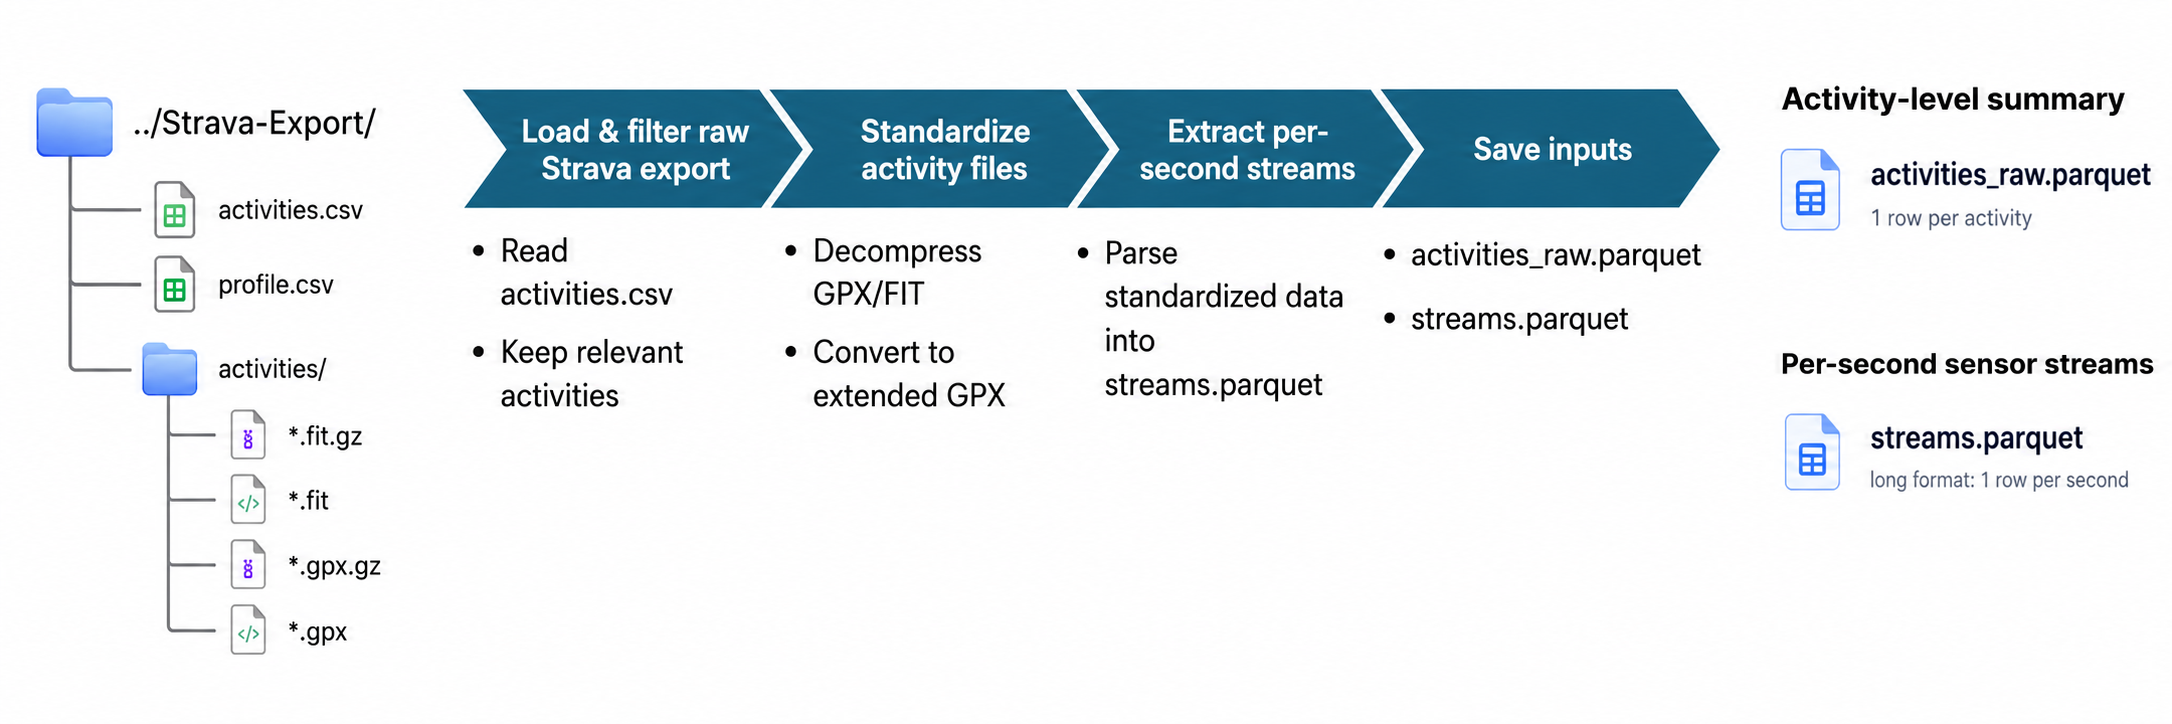
\includegraphics[width=0.95\textwidth]{graphics/data_process.png}
\end{frame}

% ----------------------------------------------------------
\begin{frame}{Activities Data Overview}

\begin{itemize}
    \item \textbf{Feature matrix}
    \begin{itemize}
        \item Final feature table: \textbf{495 rows} and \textbf{21 features}.
    \end{itemize}
\end{itemize}

\vspace{0.25cm}

\begin{center}
\begin{tabular}{l l}
\toprule
\textbf{Group} & \textbf{Variables} \\
\midrule
Volume & \texttt{distance\_km}, \texttt{moving\_s}, \texttt{mean\_gap\_speed\_mps} \\
Heart rate & \texttt{mean\_hr}, \texttt{p50\_hr}, \texttt{p90\_hr} \\
Training load & \texttt{atl}, \texttt{ctl}, \texttt{tsb} \\
Effort / calendar & \texttt{effort}, \texttt{dow}, \texttt{month} \\
\bottomrule
\end{tabular}
\end{center}

\begin{itemize}
\item \textbf{Grade-Adjusted Pace (GAP)}
    \begin{itemize}
    \item Converts observed speed to a flat-course equivalent by correcting for local slope:
        \[
        \text{GAP} = v \cdot (1 + 3.3g + 32.5g^2), \qquad
        g = \frac{\Delta \text{elevation}}{\Delta \text{distance}}
        \]
        \item $v$ = instantaneous speed; $g$ = GPS-derived gradient, clipped to reduce noise.
    \end{itemize}
\end{itemize}

\end{frame}

% ------------------------------------------------------------
\begin{frame}{Data Quality and Sample Weighting}

\textbf{Each training observation is assigned a confidence weight $w \in [0,1]$:}

\[
w = \underbrace{c_{\text{GPS}}}_{\text{valid speed}} \times
    \underbrace{c_{\text{ele}}}_{\text{valid elevation}} \times
    \underbrace{c_{\text{HR}}}_{\text{valid HR}} \times
    \underbrace{c_{\text{dur}}}_{\geq 30\,\text{min}}
\]

\vspace{0.2cm}

\begin{itemize}
    \item Each $c_i$ = fraction of per-second records with a valid sensor reading (0 = none, 1 = complete).
    \item $c_{\text{dur}}$ ramps linearly from 0 to 1 for moving time below 30 min (very short runs carry less signal).
    \item \textbf{Race rows} are pinned to $w = 1.0$ — ground-truth labels regardless of sensor dropouts.
    \item \textbf{Bonn HM (2024-04-14):} no HR strap $\Rightarrow$ HR features median-imputed from the 28-day pre-race window of other runs.
    \item All tabular models (GAM, RF, GBR, SVR) consume $w$ via \texttt{sample\_weight}; mean weight per LORO fold: 0.60--0.71.
\end{itemize}

\end{frame}

% ------------------------------------------------------------
\begin{frame}{Descriptive Summary}
\centering
\begin{columns}[T,totalwidth=\textwidth]
\begin{column}{1\textwidth}
    \centering
    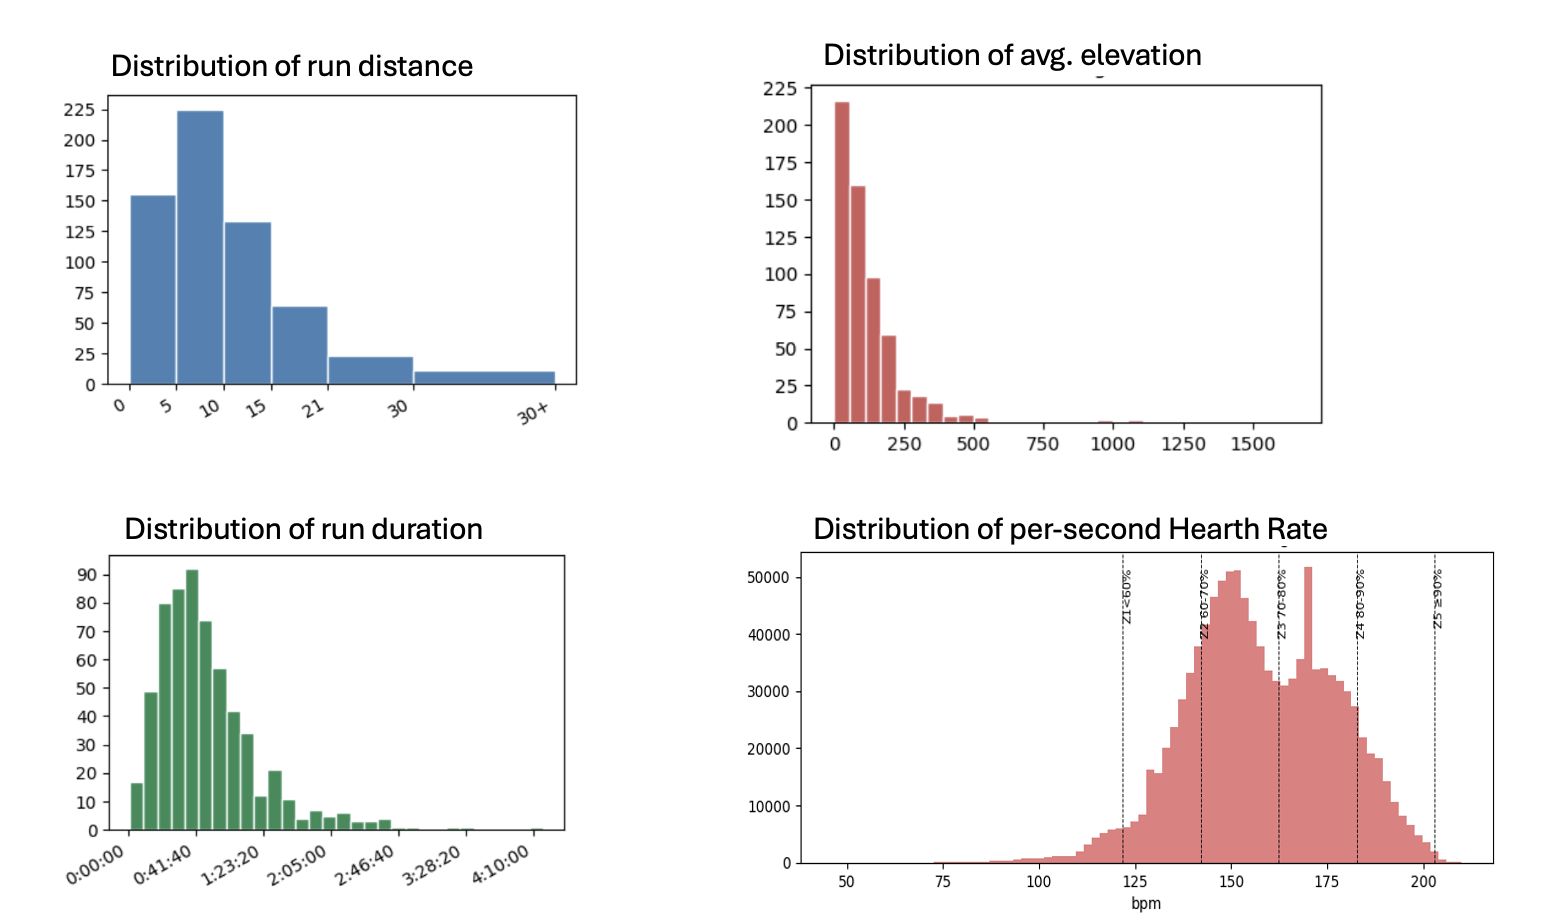
\includegraphics[width=\textwidth]{graphics/descriptive.png}
\end{column}
\end{columns}
\end{frame}

% ------------------------------------------------------------
\section{Methodology}
\subsection{Motivation: Limitations of Existing Predictors}

\begin{frame}{Commercial Race Predictors and Their Limitations}

\begin{center}
\resizebox{\textwidth}{!}{%
\begin{tabular}{l l l}
\toprule
\textbf{Platform} & \textbf{Method} & \textbf{Key Limitation} \\
\midrule
Riegel (1981)  & Power law from one reference race        & Ignores all training history \\
Strava         & Riegel-like; updates on new race         & Step function; no load sensitivity \\
Garmin         & VO\textsubscript{2}max estimate + power law & Proprietary; black-box \\
\bottomrule
\end{tabular}}
\end{center}

\textbf{Shared limitations:}
\begin{itemize}\setlength{\itemsep}{2pt}
    \item \textbf{Race-only calibration} --- hundreds of training runs discarded.
    \item \textbf{Flat-course assumption} --- same prediction regardless of course profile.
    \item \textbf{No uncertainty quantification} --- point estimate only, no prediction interval.
    \item \textbf{Opaque models} --- no interpretability beyond the formula itself.
\end{itemize}

\smallskip

{\small\raggedright\textbf{$\Rightarrow$ Our approach:} use \emph{all} training runs via pseudo-label inversion, transparent models with prediction intervals, and Minetti elevation correction.\par}

\end{frame}

\subsection{Modelling Approach}
\begin{frame}{Methodology}

\vspace{0.25cm}

\begin{enumerate}
    \item \textbf{Pseudo-label inversion}
    \begin{itemize}
        \item Each training run provides an observed pace at a known effort level.
        \[
            \text{effort} = \frac{\text{HR}}{\text{HR}_{\max}}
        \]
        \item The model learns:
        \[
            \text{pace} = f(\text{distance}, \text{effort}, \text{fitness state}, \text{calendar})
        \]
    \end{itemize}

    \vspace{0.15cm}

    \item \textbf{Temporal honesty}
    \begin{itemize}
        \item For each race, the model only uses activities recorded \textbf{before} that race date.
        \item This avoids using future training data to predict past races.
        \item Errors can therefore be interpreted as realistic race-day prediction errors.
    \end{itemize}
\end{enumerate}

\end{frame}

\subsection{Model Selection}

\begin{frame}{Methodology}

\begin{enumerate}
    \setcounter{enumi}{2}

    \item \textbf{Leave-one-race-out cross-validation}
    \begin{itemize}
        \item With six race labels, each race is held out once.
        \item The model is trained on non-race activities recorded before the held-out race.
        \item This gives one realistic prediction error per race.
    \end{itemize}

    \vspace{0.25cm}
\end{enumerate}
\end{frame}

\begin{frame}{Model Overview: GAM and Tree-Based Models}

\begin{enumerate}
    \item \textbf{Generalised Additive Model (GAM)}
    \begin{align*}
    \text{pace}
    = \beta_0
    &+ s_1(\text{dist.})
    + s_2(\overline{\text{HR}})
    + s_3(\text{GAP speed})
    + s_4(\text{TSB})\\
    &+ f(\text{dow})
    + f(\text{month})
    + \varepsilon
    \end{align*}

    \begin{itemize}
        \item Smooth terms: natural cubic splines.
        \item Regularisation selected by grid search.
    \end{itemize}

    \vspace{0.3cm}

    \item \textbf{Random Forest and Gradient Boosting}

    \vspace{0.15cm}

    \begin{itemize}
        \item \texttt{RandomForestRegressor}: 400 trees.
        \item \texttt{GradientBoostingRegressor}: 300 trees, max depth 3.
        \item Additional quantile-loss boosters at $\alpha = 0.05$ and $\alpha = 0.95$ provide a 90\% prediction interval.
    \end{itemize}

\end{enumerate}
\end{frame}

% ------------------------------------------------
\begin{frame}{Model Overview: SVR and Neural Network}

\begin{enumerate}
    \setcounter{enumi}{2}

    \item \textbf{Support Vector Regression}

    \vspace{0.15cm}

    \[
    C \in \{1, 10, 100\},
    \quad
    \gamma \in \{\text{scale}, 0.01, 0.1\},
    \quad
    \varepsilon \in \{1, 5, 10\}
    \]

    \vspace{0.15cm}

    \begin{itemize}
        \item RBF-kernel SVR inside a \texttt{StandardScaler} pipeline.
        \item Best full-table parameters: $C = 100$, $\varepsilon = 1$, $\gamma = 0.01$.
    \end{itemize}

    \vspace{0.3cm}

    \item \textbf{Convolutional Neural Network}

    \vspace{0.15cm}

    \[
    X_i \in \mathbb{R}^{4 \times T}, \quad
    \text{channels} = [\text{GAP}, \text{HR}, \text{cadence}, \text{grade}],
    \quad T = 7200
    \]

    \vspace{0.15cm}

    \begin{itemize}
        \item Preserves the per-second sequence instead of collapsing runs to summary statistics.
        \item Three \texttt{Conv1d} blocks followed by pooling, dropout, and dense layers.
        \item Loss: MSE on $\log(\text{pace})$; optimiser: AdamW, 30 epochs per fold.
    \end{itemize}

\end{enumerate}

\end{frame}
% ------------------------------------------------

\section{Results}

% ------------------------------------------------
\begin{frame}{Results: Leave-One-Race-Out Prediction Errors}

\small
\textbf{Signed prediction error in \%. Positive = predicted slower than actual.}

\vspace{0.2cm}

\resizebox{\textwidth}{!}{
\begin{tabular}{l r r r r r r r}
\toprule
\textbf{Race} & \textbf{Dist.} & \textbf{Actual} & \textbf{GAM} & \textbf{RF} & \textbf{GBR} & \textbf{SVR} & \textbf{NN} \\
\midrule
K\"{o}ln Nikolauslauf  & 10\,km  & 0:37:43 & +14.6 & +15.0 & +17.4 & +14.6 & +27.1 \\
Bonn HM$^\dagger$      & 21\,km  & 1:24:53 & +23.7 & +15.2 & +14.9 & +14.2 & $-$42.0 \\
Lousberglauf           & 5.6\,km & 0:19:58 & +38.7 & +31.6 & +33.0 & +32.1 & +13.0 \\
DIY-Triathlon          & 5\,km   & 0:21:18 & +20.3 & +35.7 & +32.2 & +42.5 & $-$12.9 \\
Schwarzwald Drachen.$^\ddagger$ & 10\,km & 0:44:57 & $-$3.9 & $-$3.2 & $-$4.3 & $-$4.0 & +118.5 \\
Milano Marathon        & 42\,km  & 2:58:16 & +12.8 & +13.1 & +13.4 & \textbf{+0.3} & +3.0 \\
\midrule
\multicolumn{3}{l}{\textbf{MAPE}}
& 19.0 & 19.0 & 19.2 & \textbf{18.0} & 36.1 \\
\bottomrule
\end{tabular}
}

\vspace{0.2cm}

\footnotesize
$^\dagger$ No HR sensor; HR features imputed. \quad
$^\ddagger$ Run after swim\,+\,bike; fatigue state outside training distribution.

\end{frame}

% ------------------------------------------------
\begin{frame}{Results: Model Comparison}

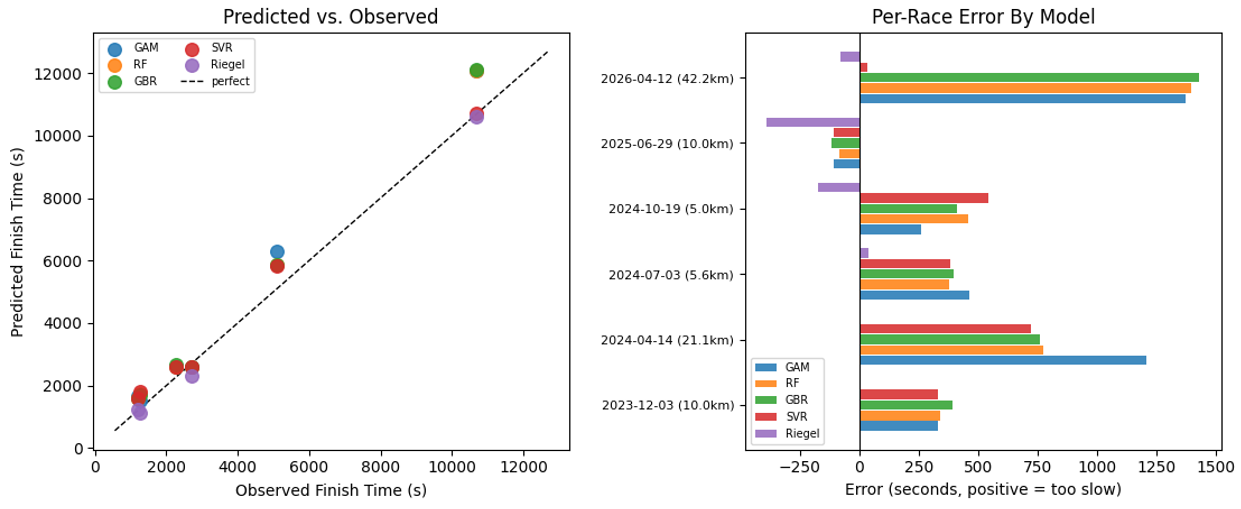
\includegraphics[width=\textwidth, height=0.50\textheight, keepaspectratio]{graphics/model_comparison.png}

\scriptsize
\begin{columns}[T]
\begin{column}{0.48\textwidth}
    \textbf{Left --- Predicted vs.\ Observed:}
    SVR sits on the identity line for the marathon; all others overshoot.
\end{column}
\begin{column}{0.48\textwidth}
    \textbf{Right --- Per-Race Error (s):}
    Marathon: SVR $\approx 0$ s; others $+1\,000$--$1\,400$ s.
    Short races: systematic over-prediction; triathlon: Riegel under-predicts.
\end{column}
\end{columns}

\end{frame}

% ------------------------------------------------
\begin{frame}{Results: Marathon Predictor --- Daily Estimates (6-Month View)}

\begin{columns}[T,totalwidth=\textwidth]

\begin{column}{0.58\textwidth}
    \centering
    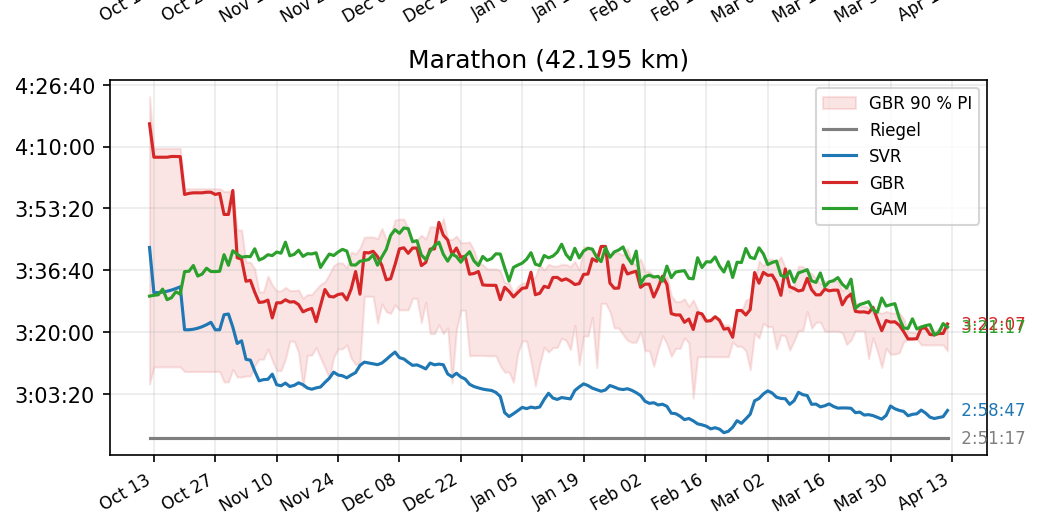
\includegraphics[width=\textwidth]{graphics/marathon_predictor.png}

    \vspace{0.1cm}
    \scriptsize
    \textbf{Riegel (grey flat line):}
    $T_2 = T_1 \cdot (D_2/D_1)^{1.06}$ \enspace (Riegel, 1981).
    Reference $(T_1, D_1)$ is unchanged between races $\Rightarrow$ constant prediction.
    Steps only when a new race is ingested; no sensitivity to daily training load.
    MAPE = 8.0\% over 4 folds --- best of all methods despite this limitation.
\end{column}

\begin{column}{0.40\textwidth}
    \footnotesize
    \begin{tabular}{l r r}
    \toprule
    \textbf{Model} & \textbf{Pred.} & \textbf{Err.} \\
    \midrule
    SVR    & 2:58:47 & +0.3\% \\
    NN$^*$ & 3:03:37 & +3.0\% \\
    Riegel & 2:56:59 & $-$0.7\% \\
    GBR    & 3:22:07 & +13.4\% \\
    GAM    & 3:21:08 & +12.8\% \\
    \midrule
    \textbf{Actual} & \textbf{2:58:16} & --- \\
    \bottomrule
    \end{tabular}

    \vspace{0.1cm}

    \scriptsize
    \begin{itemize}\setlength{\itemsep}{1pt}
        \item \textbf{SVR} (blue): 31 s off --- best model.
        \item \textbf{GBR/GAM}: $+$13\% over; PI narrows with build-up.
        \item \textbf{NN}$^*$: 2nd best (+3.0\%); not in figure.
    \end{itemize}

    \vspace{0.05cm}
    \scriptsize $^*$From LORO evaluation only.
\end{column}

\end{columns}

\end{frame}


% ------------------------------------------------
\begin{frame}{Results: Course Elevation --- Lousberglauf (5.555 km)}

\begin{columns}[T,totalwidth=\textwidth]

\begin{column}{0.55\textwidth}
    \centering
    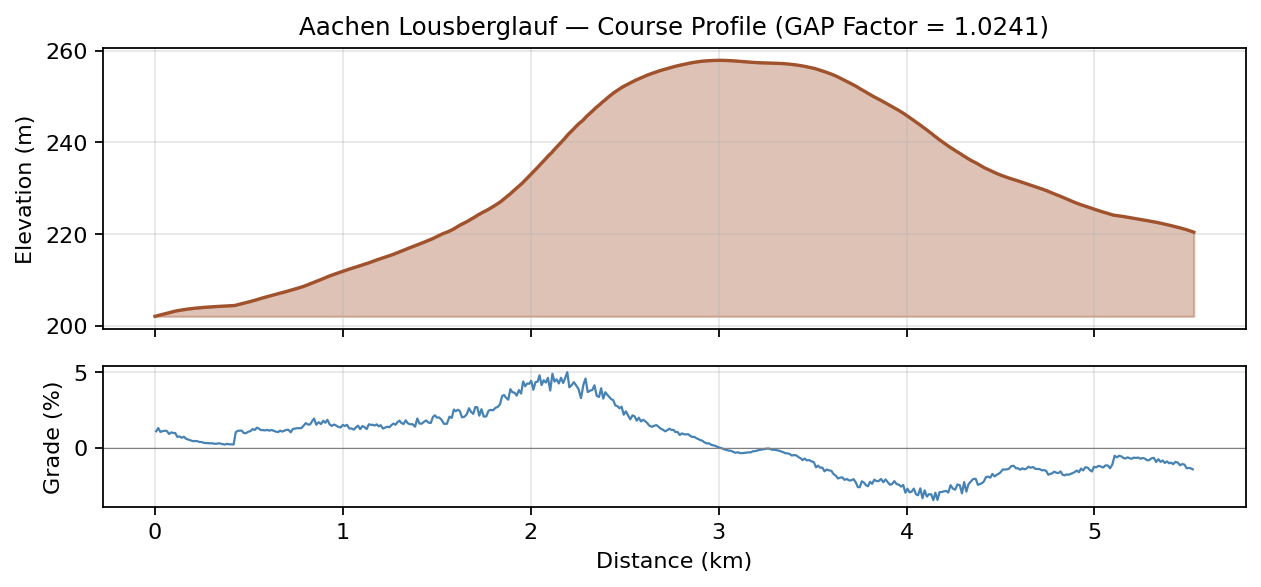
\includegraphics[width=\textwidth]{graphics/lousberglauf_profile.png}

    \vspace{0.1cm}
    \scriptsize
    \textbf{Course:} 5.53 km, $\uparrow$56 m / $\downarrow$37 m.\\
    \textbf{GAP factor} = 1.0241 (Minetti, segment-weighted) $\Rightarrow$ course is $\sim$2.4\% harder than flat.
\end{column}

\begin{column}{0.43\textwidth}
    \scriptsize
    \begin{tabular}{l r r r}
    \toprule
    \textbf{Model} & \textbf{Flat} & \textbf{Adj.} & \textbf{$\Delta$} \\
    \midrule
    GAM    & 27:42 & 28:22 & +40 s \\
    RF     & 26:17 & 26:54 & +38 s \\
    GBR    & 26:33 & 27:12 & +38 s \\
    SVR    & 26:23 & 27:01 & +38 s \\
    NN     & 22:34 & 23:06 & +33 s \\
    \midrule
    \textbf{Actual} & \multicolumn{2}{r}{\textbf{19:58}} & --- \\
    \bottomrule
    \end{tabular}

    \vspace{0.15cm}
    \scriptsize
    \begin{itemize}\setlength{\itemsep}{1pt}
        \item Models learn pace on \textbf{GAP} $\Rightarrow$ flat-course predictions.
        \item Multiplicative course correction recovers terrain effect at inference time.
        \item \textbf{Riegel, Strava, Garmin}: one number per distance, no course input.
        \item Lousberglauf gentle (+2.4\%); mountain races can exceed +15\%.
    \end{itemize}
\end{column}

\end{columns}

\end{frame}

\end{document}
